\documentclass[11pt,a4paper]{article}

\usepackage{enumerate,graphicx}
% \usepackage{../durhampaper}
\usepackage{harvard}

\usepackage{enumitem}


\addtolength{\textwidth}{2.5cm}
\addtolength{\oddsidemargin}{-1.0cm}
\addtolength{\topmargin}{-1.5cm}
\addtolength{\textheight}{2.5cm}




\citationmode{abbr}
\bibliographystyle{agsm}

\title{Generative Models for Information Security: \\ Literature Review}
\author{{\bf Student:} John Jennings  \hspace{3mm} {\bf Supervisor:} Chris Willcocks}
\date{\today}




\begin{document}

 
\maketitle 

\section *{Problem Definition}
Generative models are important tools in machine learning, seeing recent success in a wide variety of applications, from synthesizing realistic images of human faces and house interiors, to transforming photos from summer to winter and night to day. Within the information security sector, they have been used for learning novel encryption schemes, modelling password distributions, and steganography techniques for hiding information within an image. This project will expand upon current research, and investigate the applications of generative models to lexical steganography.

\section *{Definition of Terms}
\begin{itemize}[leftmargin=0pt]
\item[] \textbf{Steganography} - The art of concealed communication, differing from cryptography in that the very existence of the message is secret. This is achieved by embedding the message into a seemingly innocuous \textbf{cover text} that can be sent to the intended recipient without arousing suspicion. 

\item[] \textbf{Stegotext} - The result of steganographically embedding a message into a particular cover text.

\item[] \textbf{Lexical Steganography} - A form of steganography concerned with embedding a message within written text through the use of redundancies in natural language e.g. word ordering, inclusion of adjectives or choice of synonyms.

\item[] \textbf{Generative Model} - A model that learns the underlying distribution of the training data in order to generate new samples from the same distribution.

\end{itemize}

\section *{Identified Issues and Themes}

\subsection *{Correspondence to Neural Machine Translation}
  While the concept of lexical steganography has existed for over a decade \cite{tlex}, there has been little research conducted in the area, with almost all existing solutions employing simple techniques based on synonym substitution \cite{universal}. A thorough search of the existing literature yielded only one paper that approached the problem from a machine learning perspective, Fang et al. \citeyear{lstm}, who proposed a solution for the weaker problem of \textit{cover generation} in which the user does not have control over the content of the cover text.\\
  As a result, we will instead draw inspiration from the more mature field of Neural Machine Translation. Intuitively, lexical steganography can be thought of as a translation task, in that we are transforming the input text from one form to another while preserving the meaning. Instead of translating English text into the equivalent German text, we are translating English text into an equivalent English text that embeds the secret message.
  

\subsection *{Modelling the Problem}

  From this perspective, we can view lexical steganography as a problem of learning a generative model over the distribution of cover texts, such that given a particular cover text, we can generate new texts that are semantically equivalent. Embedding the hidden message can then be achieved through a learned algorithm that maps a particular codeword to a particular equivalent text. Decoding the hidden message from the stegotext is then simply a case of undoing this mapping.\\

  \begin{figure}[htp]
    \centering
    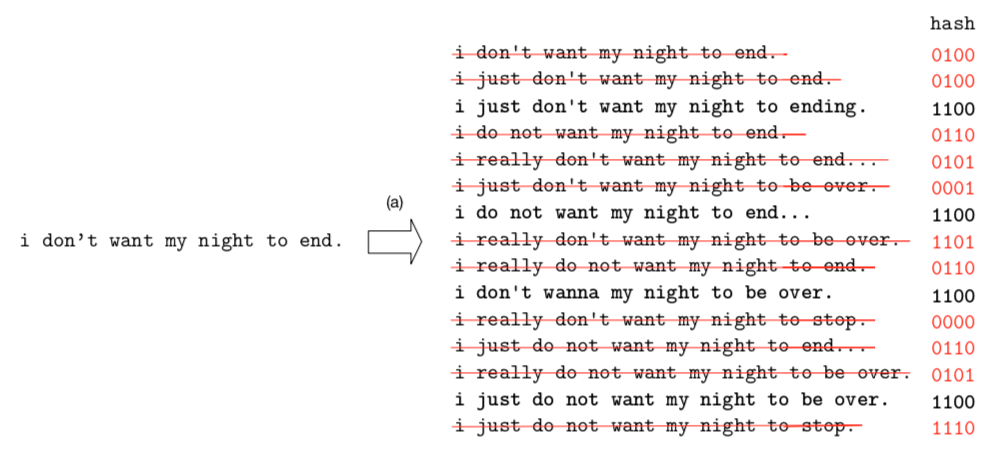
\includegraphics[width=0.9\textwidth]{mapping.png}
    \caption{An example of mapping semantically equivalent texts to codewords (Wilson et al. 2014). In this case, the codeword is determined by hashing the generated text.}
    \label{mapping}
  \end{figure}

  \nocite{covertweet1}

  \noindent We will now outline some examples of cutting-edge generative models and show how they can be modified for the purpose of lexical steganography.


  \subsubsection *{Autoencoder}
  In its simplest form, an autoencoder is a feed-forward neural network consisting of an input layer, a single hidden layer, and an output layer of the same size as the input. The model is then trained to output a reconstruction of the original input, thereby learning a latent representation of the input within the hidden layer. Modified versions of this relatively simple model have been successfully used for a number of applications, such as variable-rate image compression \cite{autoencimagecomp} and pretraining deep neural networks to have meaningful starting weights \cite{autoencstacking}. Compared to more traditional methods of unsupervised representation learning, such as principal component analysis, the autoencoder is shown to have a better expressive power, due to its ability to learn non-linear encodings \cite{goodfellow}.\\
  \indent One type of autoencoder that is of particular use for lexical steganography is the variational autoencoder (VAE), which learns to encode a training sample as a probability distribution over the latent space, instead of a single point. This is effective in generalizing the autoencoder to act as a generative model over the training distribution. In the case of lexical steganography, a VAE could be trained on a set of cover texts such that at inference time, sampling from the distribution of a particular cover text will yield equivalent texts that can then each be mapped to a codeword.
  
  seq2seq
  seqgan

  char/word/tweet level






\subsection *{Dataset}
  For training 


% we basically just need a lot of english text, no need for labels etc
% lots of choice 
% everybody uses twitter for good reason
%   pretty standard form compared to prose
%   character limit <- good since RNNs tend to struggle on longer sequences
%   lots of data available
%   can compare against existing solutions
%   misspellings + slang -> more synonyms
%   has an immediate use case


\subsection *{Additional tuning}
  word embeddings
  skip connections
  dropout

\subsection *{Loss Function}
  nll vs bleu

\section *{Proposed Direction of the Project}

\bigskip


\bibliography{../bib}
\end{document} 